\section{Pendahuluan}
Pada modul ini, kita akan membahas konfigurasi routing static dan routing dinamis pada perangkat
MikroTik. Routing merupakan proses pengiriman data antara dua atau lebih jaringan yang berbeda.
\\ \\ \indent Dalam modul ini, kita akan membahas konsep dasar routing, macam-macam routing statis dan dinamis, serta langkah-langkah untuk mengkonfigurasi kedua jenis routing ini pada perangkat MikroTik.
\\ \\ \indent Sebelum memulai pembahasan routing, penting untuk memahami konsep dasar jaringan dan subnetting. Jaringan terdiri dari sejumlah perangkat yang terhubung satu sama lain, seperti komputer,
printer, dan perangkat jaringan lainnya. Setiap perangkat dalam jaringan memiliki alamat IP yang unik.
\\ \\ \indent Subnetting adalah proses pembagian jaringan menjadi subnet yang lebih kecil. Dengan subnetting,
kita dapat mengoptimalkan penggunaan alamat IP dan membagi jaringan menjadi beberapa segmen
yang terpisah.
\\ \\ \indent Dalam routing, terdapat yang namanya protokol routing. Protokol routing adalah aturan yang digunakan oleh perangkat jaringan untuk memilih jalur terbaik bagi pengiriman data antara jaringan yang
berbeda. Ada dua jenis protokol routing utama: routing static dan routing dinamis.

%===========================================================%

\section{Tujuan Praktikum}
Mengetahui dan memahami konfigurasi routing static dan routing dinamis pada Mikrotik. Serta Dapat mengkonfigurasi konfigurasi routing static dan routing dinamis pada Mikrotik dengan tepat.
%===========================================================%

\section{Alat dan Bahan}
\begin{itemize}[label=$\bullet$, itemsep=-1pt, leftmargin=*]
	\item 2 perangkat router mikrotik.
	\item Aplikasi Winbox.
	\item 3 kabel LAN
\end{itemize}
%===========================================================%

\section{Langkah-langkah Percobaan}
\textbf{gambar pada langkah-langkah di bagian ini akan diisi gambar contoh dari template dulu,
		karena nanti akan kami ganti dengan screenshot langkah-langkah kami saat praktikum}

\subsection{Routing Statis}
Pada routing statis, terdapat setidaknya 2 jenis, yaitu :
\begin{enumerate}
	\item Default Route : digunakan ketika tidak ada rute spesifik yang cocok untuk tujuan pengiriman data. Jika tidak ada rute yang cocok, paket data akan dikirim melalui default route. Pada MikroTik,
	default route dinyatakan sebagai 0.0.0.0/0.
	\item Static Route : adalah jenis routing di mana administrator jaringan secara manual mengonfigurasi
	tabel routing pada setiap perangkat jaringan. Dalam routing static, rute yang ditentukan secara
	manual digunakan untuk mengarahkan paket data ke tujuan yang ditentukan.
\end{enumerate}

%Langkah untuk konfigurasi Router 1
\begin{center} 
	\textbf{Konfigurasi Router 1}
\end{center}

\begin{enumerate}
	% poin 1
	\item Buka aplikasi WinBox pada PC 1 dan lakukan koneksi ke Router 1. Neighbors > Refresh >
	Double click Router yang terdeteksi > Connect
	\begin{figure}[H]
		\centering
		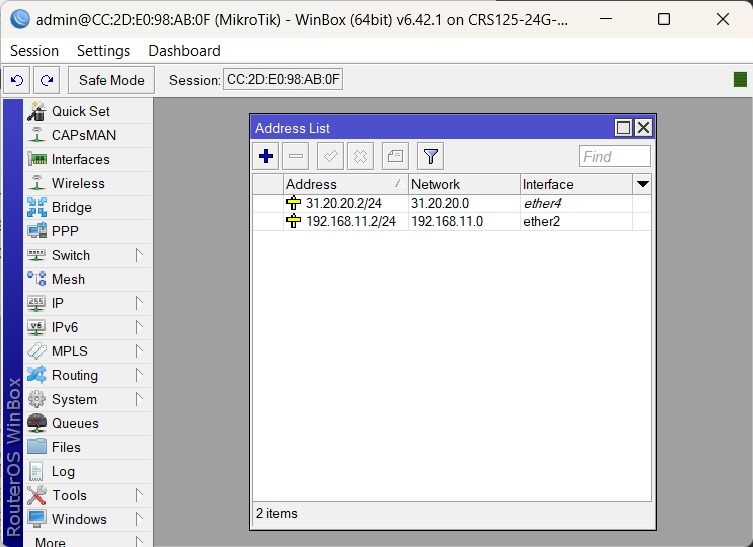
\includegraphics[width=0.5\linewidth]{P2/img/statis_R1step1.jpg}
		\caption{Step 1}
		\label{fig:gambar1}
	\end{figure}

	% poin 2
	\item Berikan IP address pada interface ether2 dan ether 4 yang dapat dibuat pada tab IP > Addresses. Berikan IP address sesuai dengan cara pengaturan IP address yang benar. Berikan IP
	address yang berbeda dengan contoh di modul.
	\begin{figure}[H]
		\centering
		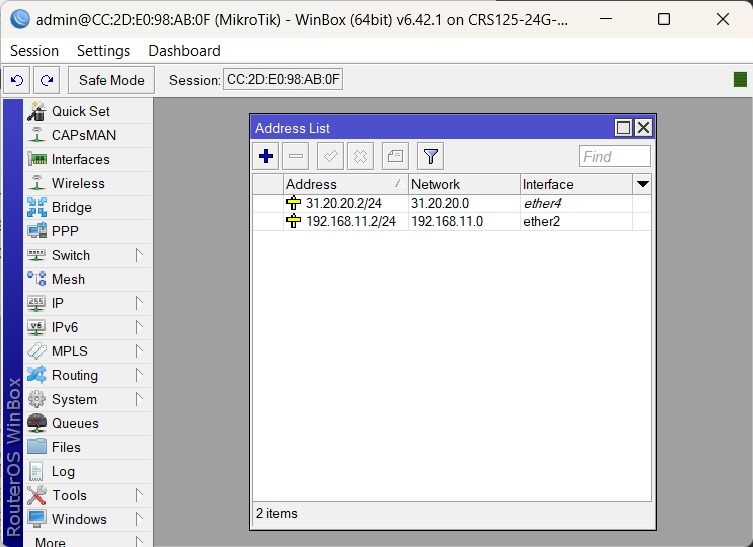
\includegraphics[width=0.5\linewidth]{P2/img/statis_R1step1.jpg}
		\caption{Step 2}
		\label{fig:gambar2}
	\end{figure}

	% poin 3.1
	\item Lakukan routing statis. Buka pada tab IP > Routes, lalu tambahkan jaringan.
	\begin{figure}[H]
		\centering
		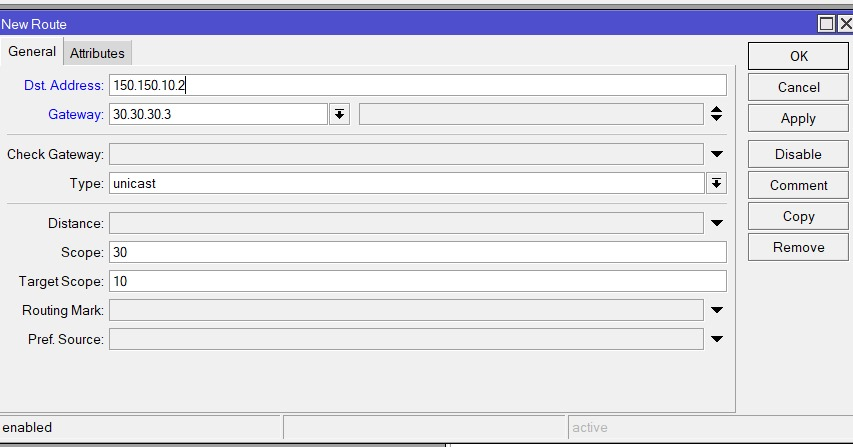
\includegraphics[width=0.5\linewidth]{P2/img/statis_R1step3.jpg}
		\caption{Step 3.1}
		\label{fig:gambar3}
	\end{figure}

	% poin 3.2
	Masukkan alamat jaringan yang ingin dituju, melalui alamat Gateway pada router 2
	
	\begin{figure}[H]
		\centering
		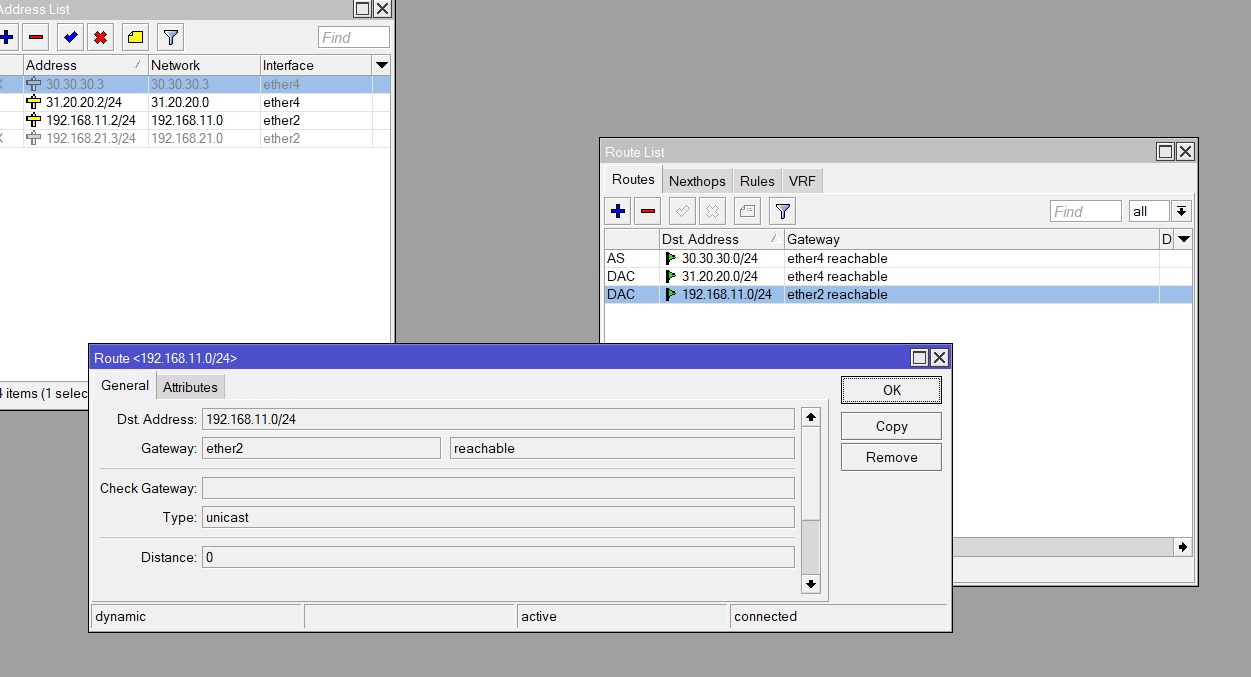
\includegraphics[width=0.5\linewidth]{P2/img/statis_R1step3.2.jpg}
		\caption{Step 3.2}
		\label{fig:gambar4}
	\end{figure}

\end{enumerate}

%Langkah untuk konfigurasi Router 2
\begin{center} 
	\textbf{Konfigurasi Router 2}
\end{center}

\begin{enumerate}
	% poin 1
	\item Buka WinBox dan lakukan koneksi ke Router 2

	% poin 2
	\item Berikan IP address pada interface ether2 dan ether 4 yang dapat dibuat pada tab IP > Addresses. Berikan IP address sesuai dengan cara pengaturan IP address yang benar. Berikan IP
	address yang berbeda dengan contoh di modul.
	\begin{figure}[H]
		\centering
		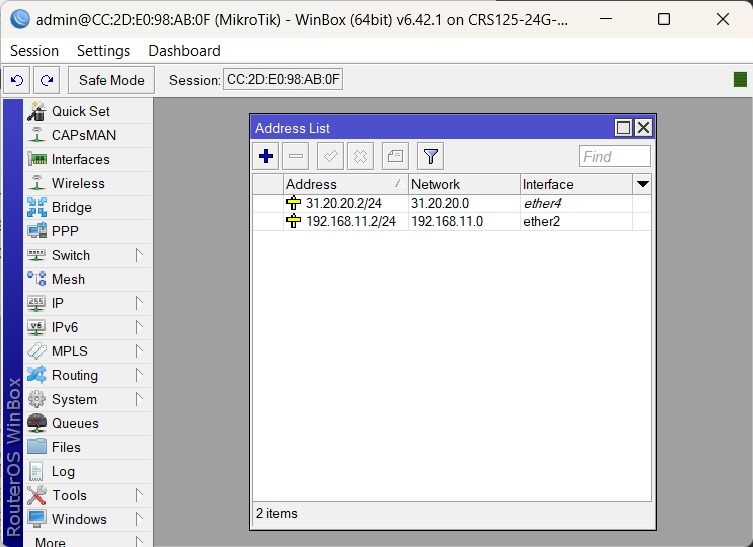
\includegraphics[width=0.5\linewidth]{P2/img/statis_R1step1.jpg}
		\caption{Step 2}
		\label{fig:gambar6}
	\end{figure}

	% poin 3
	\item Lakukan routing statis. Buka pada tab IP > Routes, lalu tambahkan jaringan. Masukkan alamat
	jaringan yang ingin dituju, melalui alamat Gateway pada router 1
	\begin{figure}[H]
		\centering
		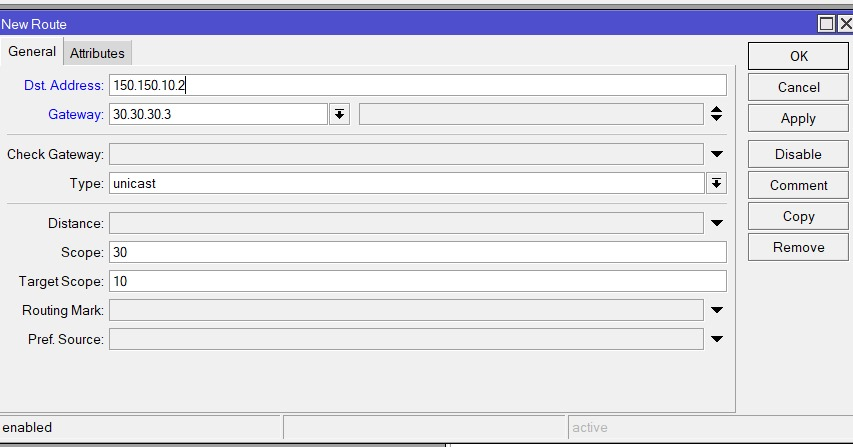
\includegraphics[width=0.5\linewidth]{P2/img/statis_R1step3.jpg}
		\caption{Step 3}
		\label{fig:gambar7}
	\end{figure}

\end{enumerate}

%Langkah untuk Mengecek keberhasilan konfigurasi
\begin{center} 
	\textbf{Mengecek keberhasilan konfigurasi}
\end{center}

\begin{enumerate}
	% poin 1
	\item Lakukan tes ping ke Router 2 melalui PC 1
	\begin{figure}[H]
		\centering
		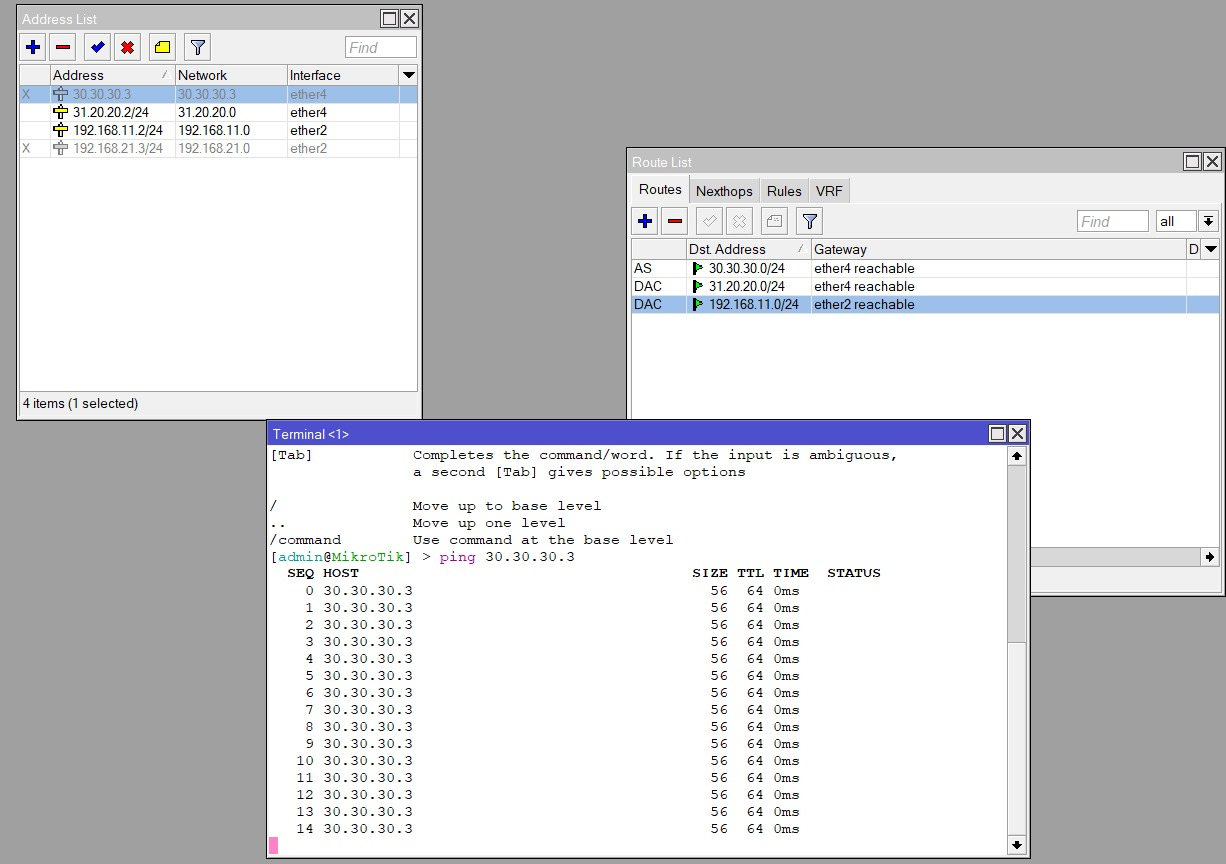
\includegraphics[width=0.5\linewidth]{P2/img/statis_ping.jpg}
		\caption{Step 1}
		\label{fig:gambar8}
	\end{figure}

	% poin 2
	\item Lakukan tes ping ke Router 1 melalui PC 2
	\begin{figure}[H]
		\centering
		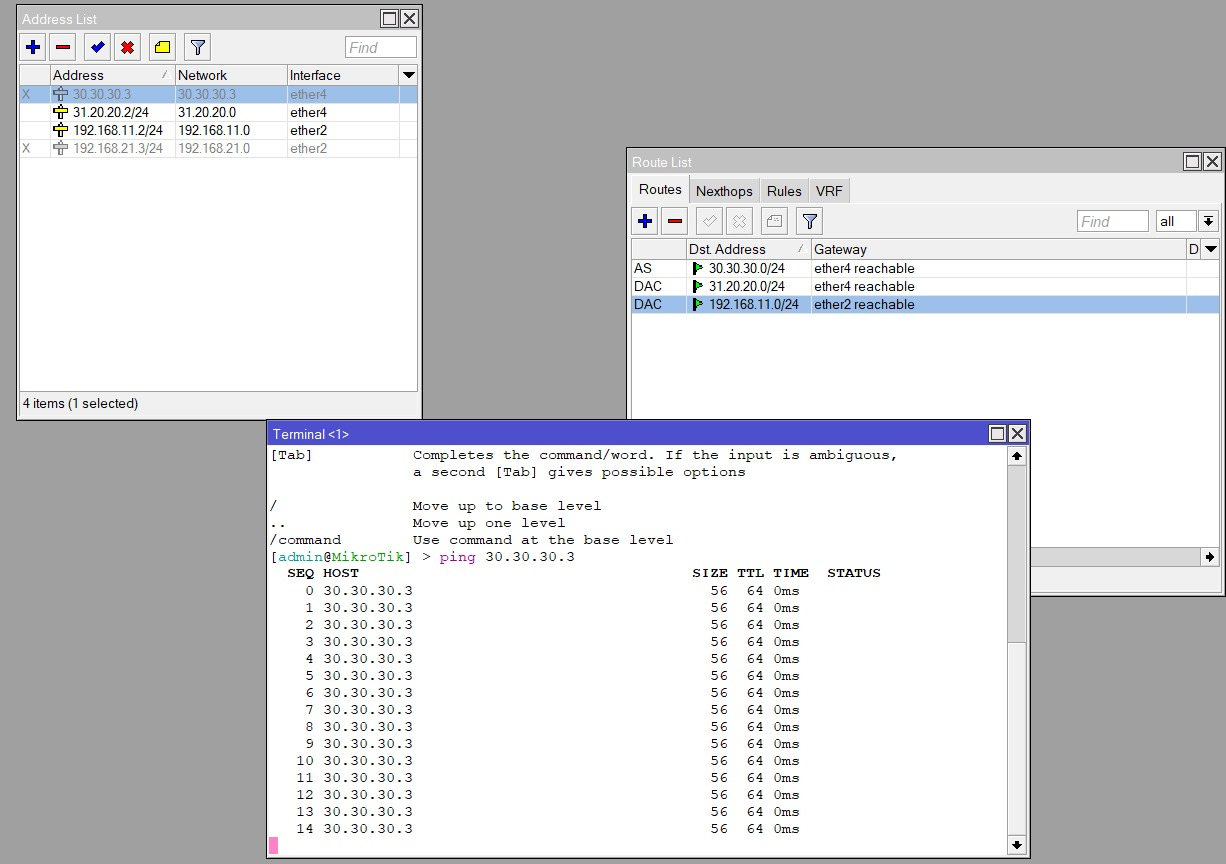
\includegraphics[width=0.5\linewidth]{P2/img/statis_ping.jpg}
		\caption{Step 2}
		\label{fig:gambar9}
	\end{figure}

\end{enumerate}

\subsection{Routing Dinamis}
Pada routing dinamis, terdapat setidaknya 3 jenis, yaitu :
\begin{enumerate}
	\item Routing Information Protocol (RIP) RIP adalah salah satu protokol routing dinamis yang menggunakan metrik hop count (jumlah hop) untuk menentukan jalur terbaik. Metrik hop count mengukur jarak antara router pengirim dengan tujuan dalam jumlah hop (melalui berapa banyak router).
	\item Open Shortest Path First (OSPF) OSPF adalah protokol routing dinamis yang menggunakan
	algoritma Dijkstra untuk menentukan jalur terpendek. OSPF mengumpulkan informasi topologi
	dari semua router dalam jaringan dan menghitung jalur terbaik berdasarkan bobot (cost) setiap
	link.
	Border Gateway Protocol (BGP) BGP adalah protokol routing eksternal yang digunakan di Internet. BGP memungkinkan router di AS (Autonomous System) yang berbeda untuk berkomunikasi dan menukar informasi routing
\end{enumerate}

%Langkah untuk konfigurasi Router 1
\begin{center} 
	\textbf{Konfigurasi Router 1}
\end{center}

\begin{enumerate}
	% poin 1
	\item Buka WinBox dan lakukan koneksi ke Router 1

	% poin 2
	\item Berikan IP address pada interface ether2 dan ether 4 yang dapat dibuat pada tab IP > Addresses. Berikan IP address sesuai dengan cara pengaturan IP address yang benar Berikan IP
	address yang berbeda dengan contoh di modul.
	\begin{figure}[H]
		\centering
		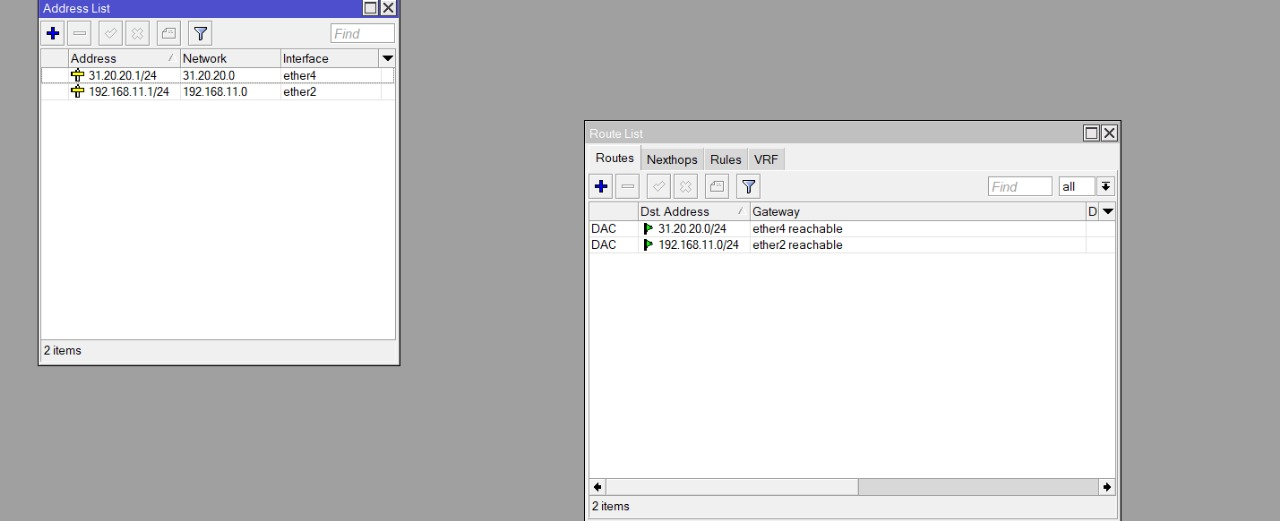
\includegraphics[width=0.5\linewidth]{P2/img/dinamis_R1step2.jpg}
		\caption{Step 2}
		\label{fig:gambar11}
	\end{figure}

	% poin 3.1
	\item Pada PC 1, lakukan routing dinamis. Buka tab Routing > RIP.
	\begin{figure}[H]
		\centering
		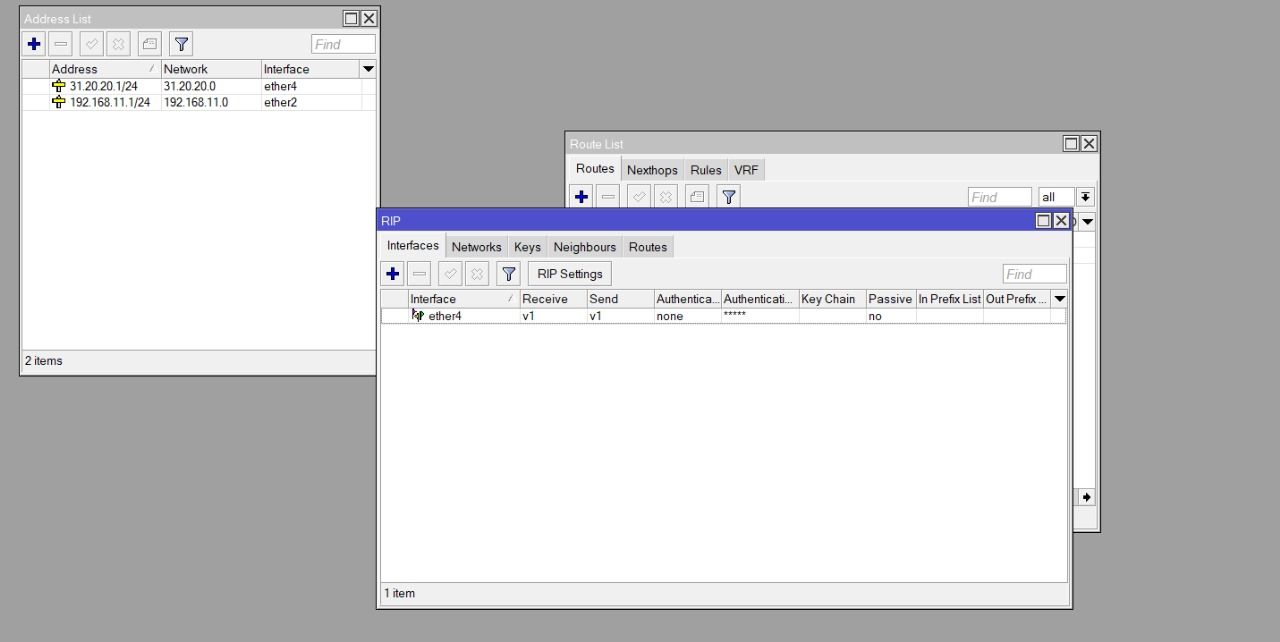
\includegraphics[width=0.5\linewidth]{P2/img/dinamis_R1step3.1.jpg}
		\caption{Step 3.1}
		\label{fig:gambar38}
	\end{figure}

	% poin 3.2
	Pada interface tambahkan interface baru kemudian ubah interface menjadi ether 4 dengan Receive dan Send pada v1.
	\begin{figure}[H]
		\centering
		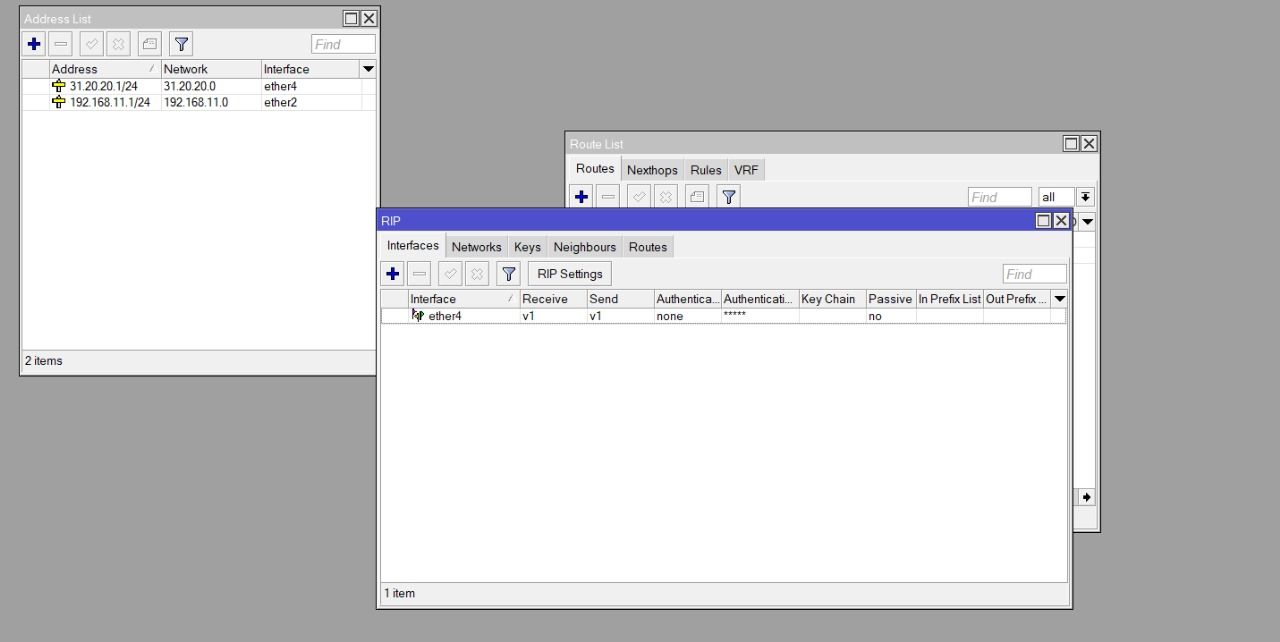
\includegraphics[width=0.5\linewidth]{P2/img/dinamis_R1step3.1.jpg}
		\caption{Step 3.2}
		\label{fig:gambar39}
	\end{figure}

	% poin 4
	\item Pada tab Network, tambahkan 2 network baru, yaitu network yang antara PC1 dengan Router
	1 dan network antara Router 1 dan Router 2.	
	\begin{figure}[H]
		\centering
		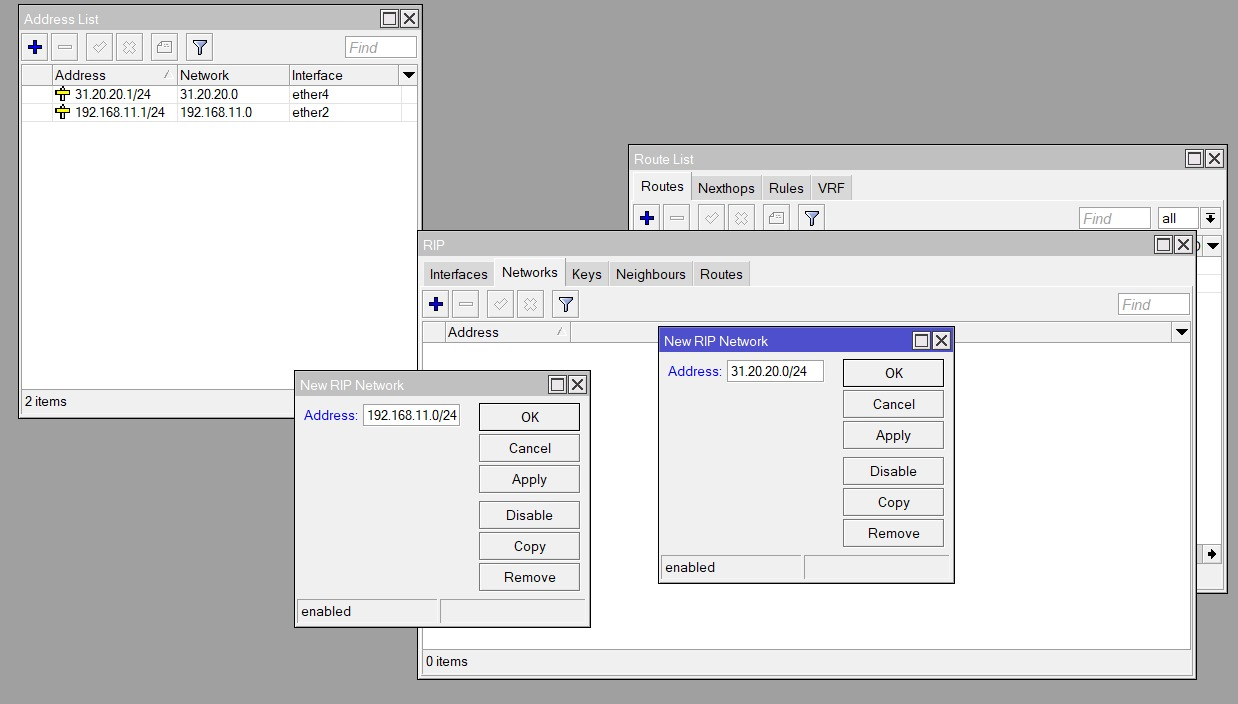
\includegraphics[width=0.5\linewidth]{P2/img/dinamis_R1step3.2.jpg}
		\caption{Step 4}
		\label{fig:gambar38}
	\end{figure}

	% poin 5
	\item Pada tab Neighbours, tambahkan alamat router yang dituju.
	\begin{figure}[H]
		\centering
		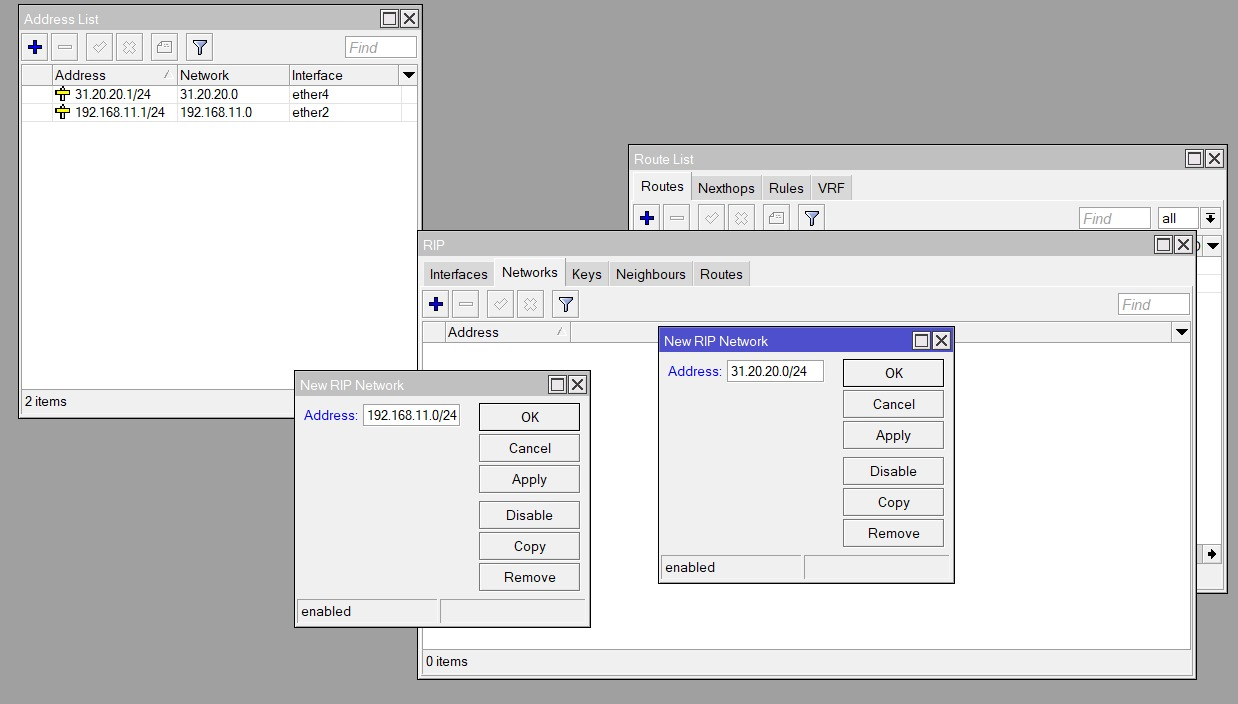
\includegraphics[width=0.5\linewidth]{P2/img/dinamis_R1step3.2.jpg}
		\caption{Step 5}
		\label{fig:gambar38}
	\end{figure}

\end{enumerate}

%Langkah untuk konfigurasi Router 2
\begin{center} 
	\textbf{Konfigurasi Router 2}
\end{center}

\begin{enumerate}
	% poin 1
	\item Buka WinBox dan lakukan koneksi ke Router 2
	
	% poin 2
	\item Berikan IP address pada interface ether2 dan ether 4 yang dapat dibuat pada tab IP > Addresses. Berikan IP address sesuai dengan cara pengaturan IP address yang benar. Berikan IP
	address yang berbeda dengan contoh di modul.
	\begin{figure}[H]
		\centering
		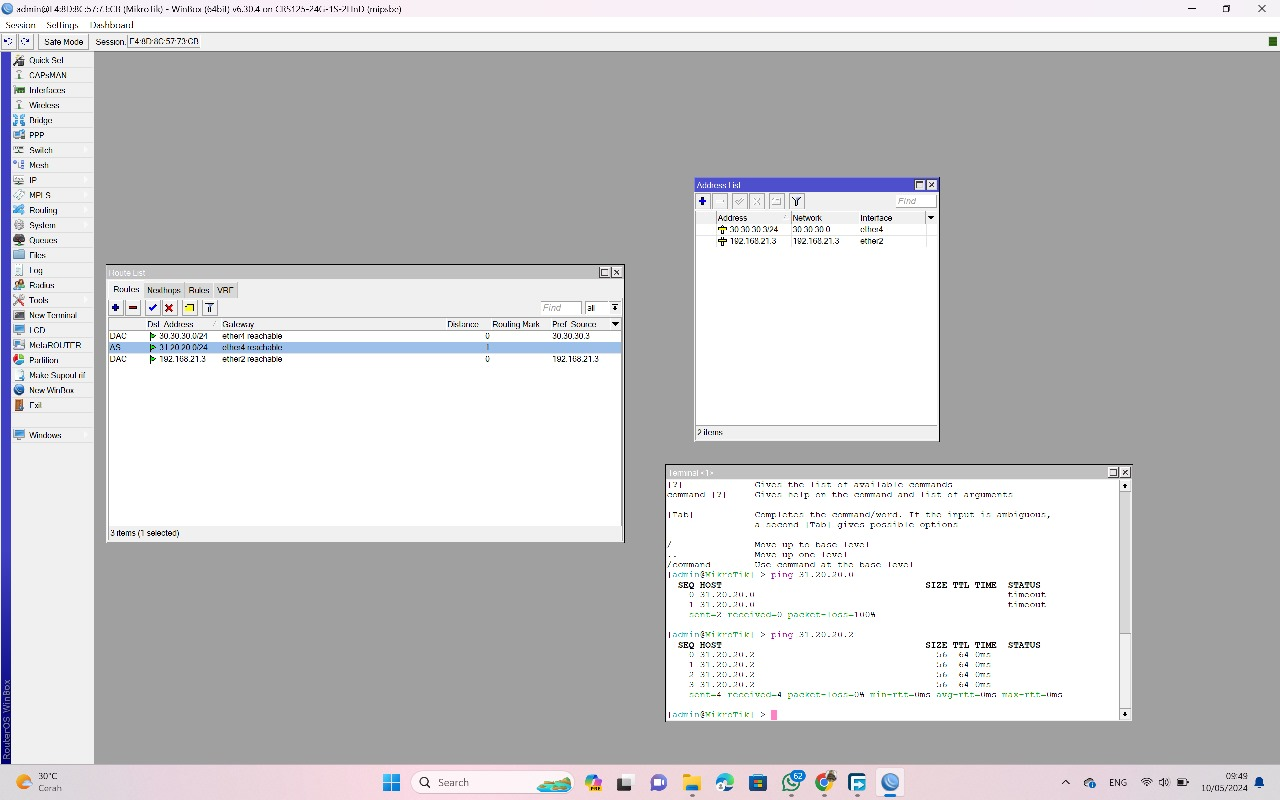
\includegraphics[width=0.5\linewidth]{P2/img/dinamis_R2step2.jpg}
		\caption{Step 2}
		\label{fig:gambar13}
	\end{figure}
	
	% poin 3
	\item Pada tab Network, tambahkan 2 network baru, yaitu network yang antara PC2 dengan Router
	2 dan network antara Router 1 dan Router 2.
	\begin{figure}[H]
		\centering
		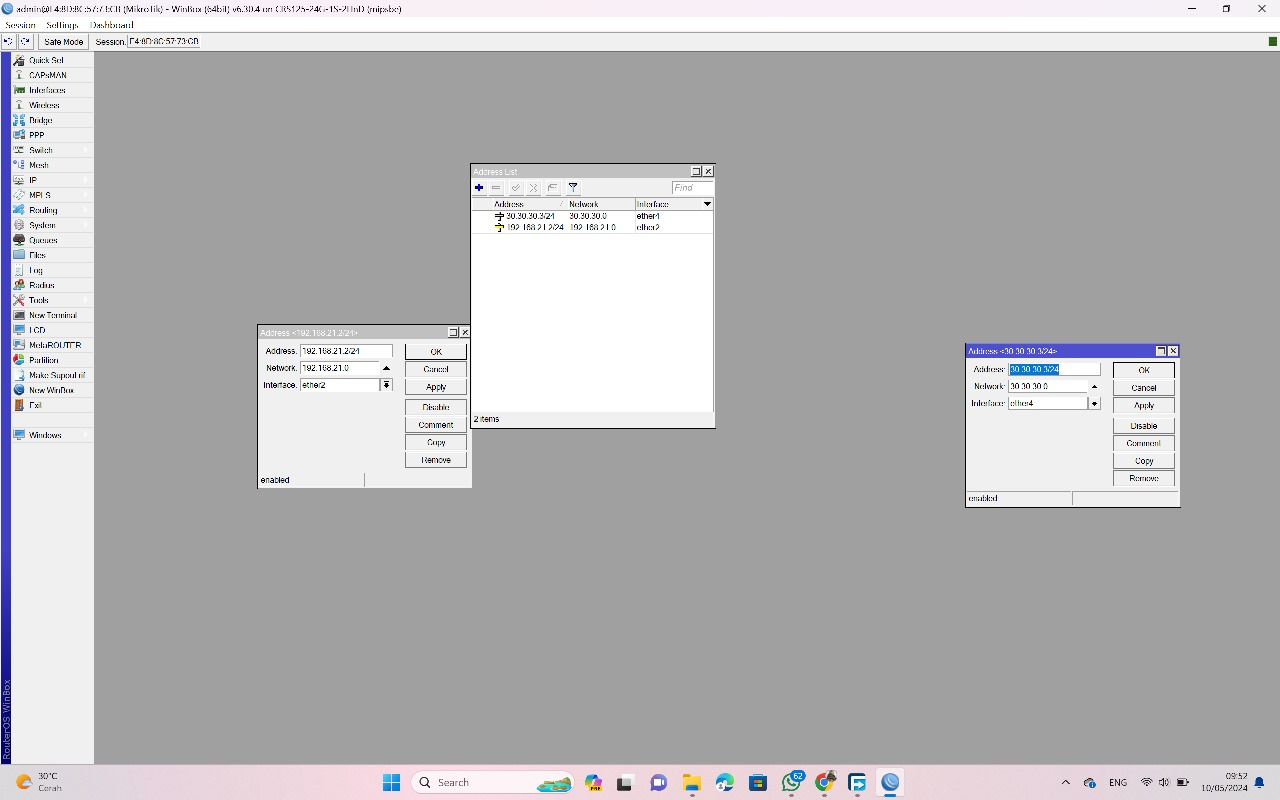
\includegraphics[width=0.5\linewidth]{P2/img/dinamis_R2step3.2.jpg}
		\caption{Step 3}
		\label{fig:gambar13}
	\end{figure}

	% poin 4
	\item Pada tab Neighbours, tambahkan alamat router yang dituju.
	\begin{figure}[H]
		\centering
		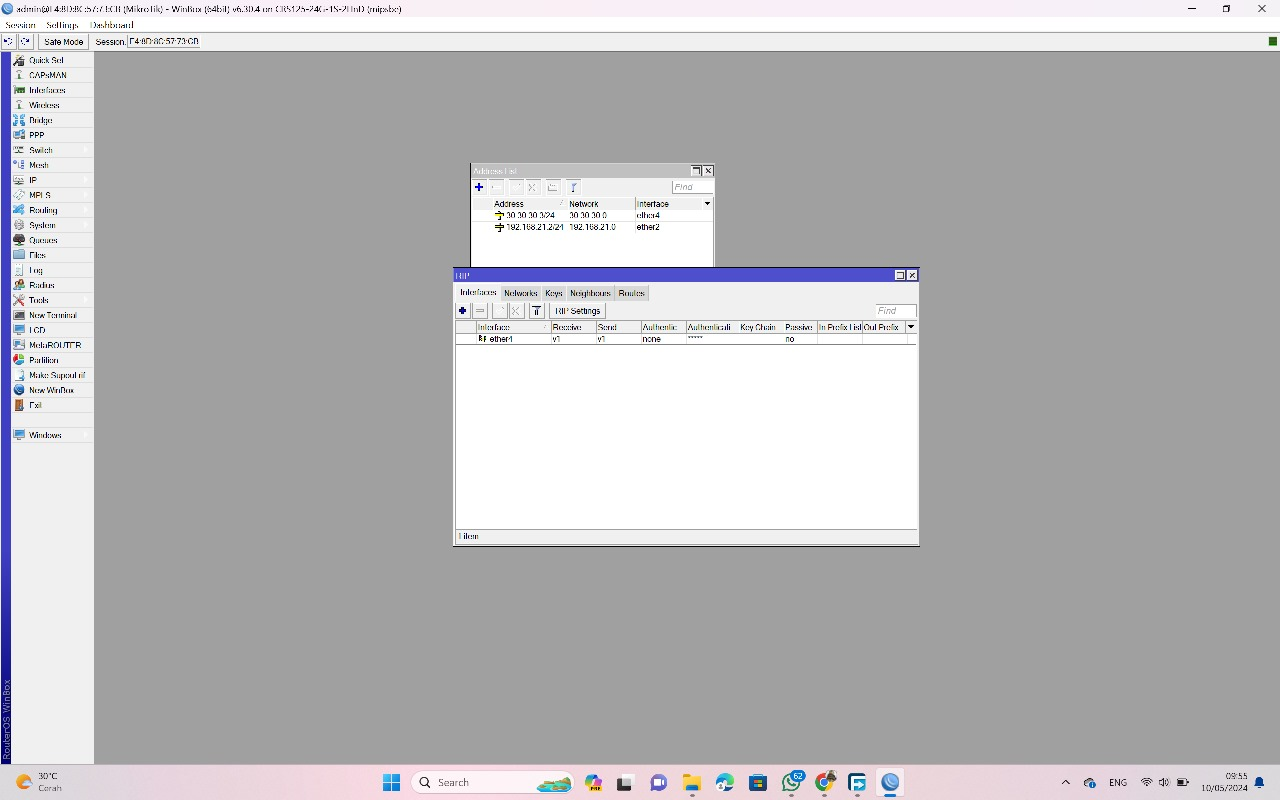
\includegraphics[width=0.5\linewidth]{P2/img/dinamis_R2step4.jpg}
		\caption{Step 4}
		\label{fig:gambar13}
	\end{figure}

\end{enumerate}

%Langkah untuk Mengecek keberhasilan konfigurasi
\begin{center} 
	\textbf{Mengecek keberhasilan konfigurasi}
\end{center}

\begin{enumerate}
	% poin 1
	\item Lakukan tes ping Router 2 dari PC 1
	\begin{figure}[H]
		\centering
		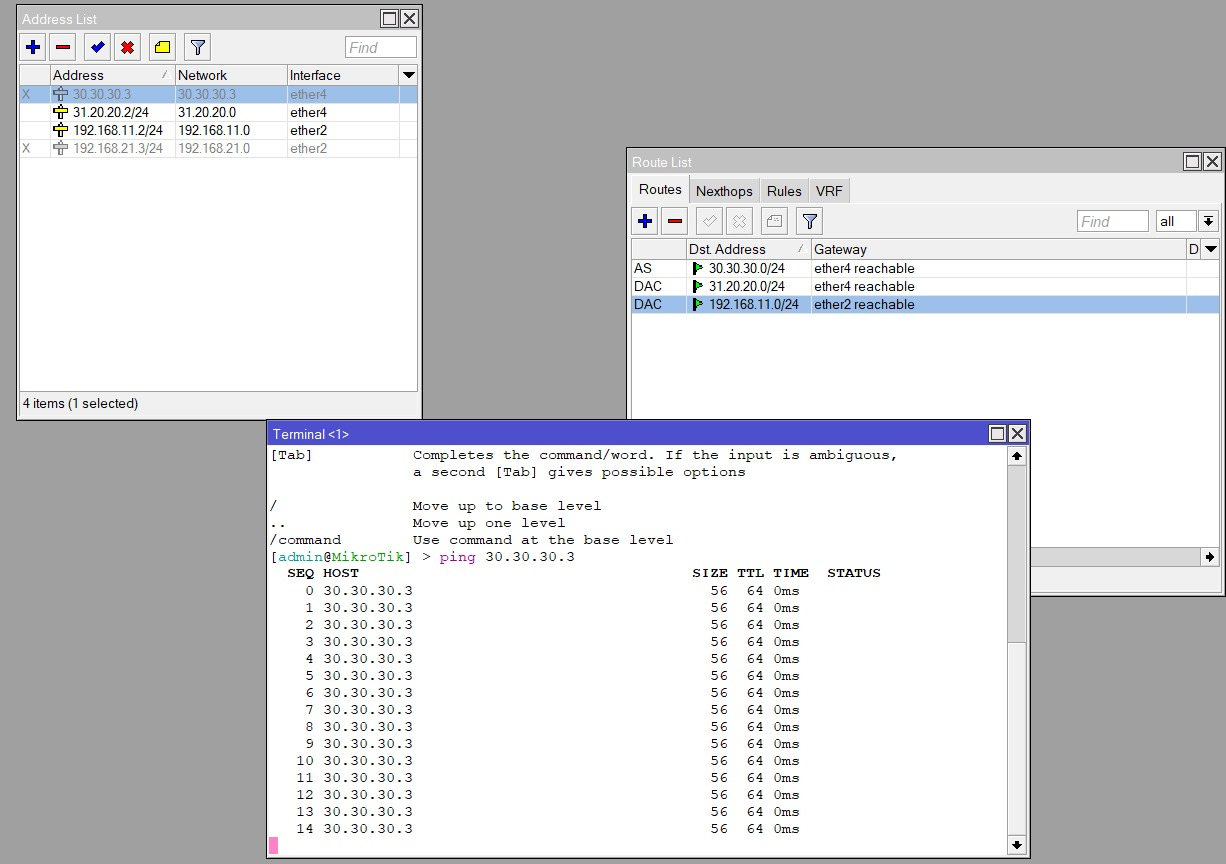
\includegraphics[width=0.5\linewidth]{P2/img/statis_ping.jpg}
		\caption{Step 1}
		\label{fig:gambar14}
	\end{figure}

	% poin 2
	\item Lakukan tes ping Router 1 dari PC 2
	\begin{figure}[H]
		\centering
		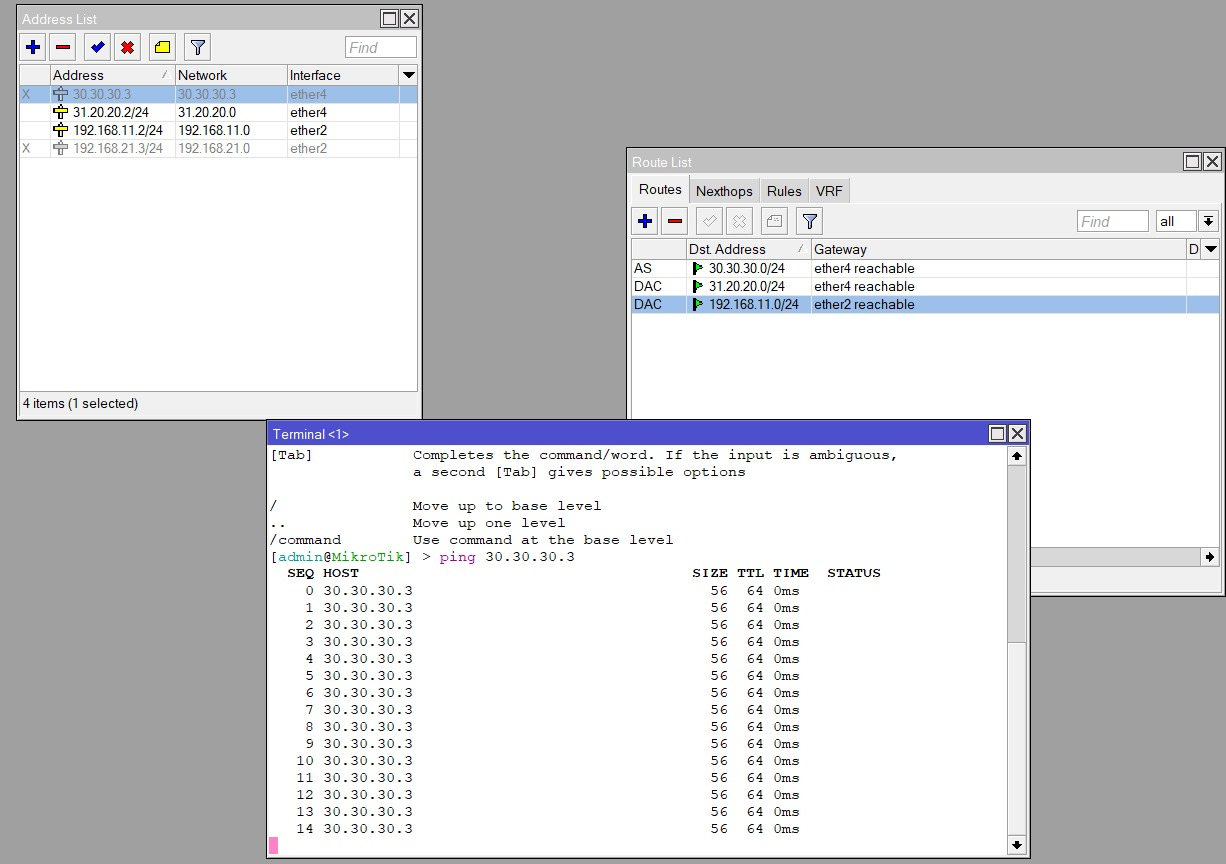
\includegraphics[width=0.5\linewidth]{P2/img/statis_ping.jpg}
		\caption{Step 2}
		\label{fig:gambar15}
	\end{figure}

\end{enumerate}

\section{Hasil Percobaan}
Hasil percobaan yang didapat dari modul 2 adalah terhubungnya 2 router dengan 2 laptop menggunakan teknik routing statis dan routing dinamis. Pada routing statis diperlukan penambahan setiap jaringan yang akan dituju sedangkan pada routing dinamis jaringan yang ditambahkan hanya jaringan yang diketahui oleh router saja.
%===========================================================%

\section{Kesimpulan}
Kesimpulan dari modul ini adalah bahwa konfigurasi routing statis dan dinamis pada perangkat MikroTik memerlukan pemahaman dasar mengenai pengaturan IP Address dan subnetting. Pada routing statis, administrator jaringan secara manual menentukan rute untuk mengarahkan paket data, sedangkan pada routing dinamis, seperti RIP, protokol secara otomatis menentukan jalur terbaik berdasarkan metrik tertentu.raktikum ini memberikan pemahaman yang mendalam tentang bagaimana mengonfigurasi dan mengelola routing pada perangkat MikroTik, sehingga peserta dapat mengimplementasikan routing yang efektif dalam jaringan mereka.
%===========================================================%

\section{Lampiran}

\subsection{Tugas Pendahuluan}
\begin{enumerate}
	\item Buatlah topologi jaringan percobaan 1 dan 2!
	\begin{itemize}
		\item Topologi jaringan percobaan 1
		\begin{figure}[H]
		\centering
		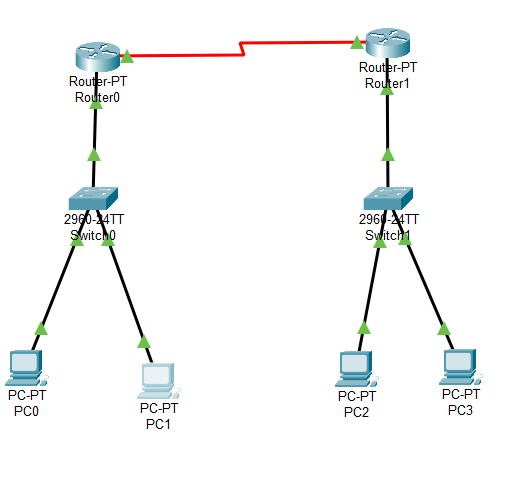
\includegraphics[width=0.75\linewidth]{P2/img/topologi1.jpg}
		\caption{Topologi Jaringan Percobaan 1}
		\label{fig:gambar31}
		\end{figure}
	
		\item Topologi jaringan percobaan 2
		\begin{figure}[H]
			\centering
			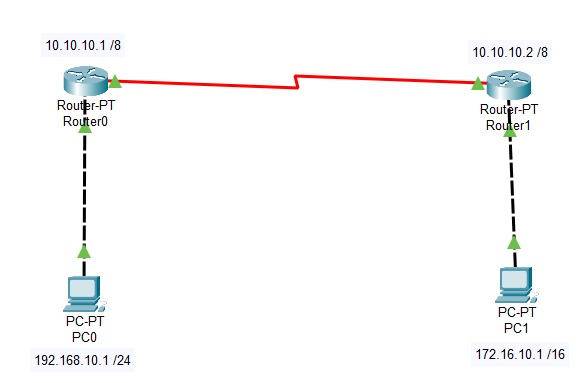
\includegraphics[width=0.75\linewidth]{P2/img/topologi2.jpg}
			\caption{Topologi Jaringan Percobaan 2}
			\label{fig:gambar32}
		\end{figure}
	\end{itemize}
	

	\item Perbedaan Static Routing dan Dynamic Routing.
	\\ Perbedaan utama antara routing statis (static routing) dan routing dinamis (dynamic routing) adalah cara mereka mengatur jalur data dalam jaringan komputer
	\begin{itemize}
		\item Static Routing
		\begin{itemize}
			\item Proses setting router jaringan menggunakan tabel routing yang dikonfigurasikan secara manual oleh administrator jaringan.
			\item Administrator harus memasukkan atau menghapus rute statis jika terjadi perubahan topologi jaringan.
		\end{itemize}

		\item Dynamic Routing
		\begin{itemize}
			\item Mampu membuat tabel routing secara otomatis berdasarkan lalu lintas jaringan dan router yang terhubung.
			\item Routing dinamis menggunakan protokol routing yang akan mengatur router secara otomatis untuk saling berkomunikasi dengan memberikan informasi tentang jaringan dan koneksi antar router.
		\end{itemize}

		
	\end{itemize}

	\item Keuntungan dan kekurangan Static Routing dan Dynamic Routing
	\begin{enumerate}
		\item Static Routing
		\begin{itemize}
			\item Kelebihan :
			\begin{itemize}
				\item[\ding{58}] Mengurangi kinerja CPU router karena pemrosesan didistribusikan ke setiap router.
				\item[\ding{58}] Penghematan bandwidth karena tidak ada bandwidth yang terbuang saat bertukar paket.
				\item[\ding{58}] Dapatkan informasi dari isi tabel routing selama pertukaran paket.
				\item[\ding{58}] Routing statis lebih aman.
				\item[\ding{58}] Administrator bebas menentukan jalur jaringan.
			\end{itemize}

			\item Kekurangan :
			\begin{itemize}
				\item[\ding{56}] Administrator jaringan harus mengetahui semua informasi tentang router yang terhubung.
				\item[\ding{56}] Jaringan kecil saja.
				\item[\ding{56}] Konfigurasi lebih rumit terutama jika beberapa komputer terhubung.
				\item[\ding{56}] Memerlukan waktu setup yang lebih lama.
				\item[\ding{56}] Jika jalur terputus, jaringan berhenti.
			\end{itemize}
		\end{itemize}

		\item Dynamic Routing
		\begin{itemize}
			\item Kelebihan :
			\begin{itemize}
				\item[\ding{58}] Cocok untuk jaringan dengan jangkauan yang lebih luas.
				\item[\ding{58}] Konfigurasi jaringan lebih cepat.
				\item[\ding{58}] Jalur ditentukan secara otomatis oleh sistem.
				\item[\ding{58}] Melindungi kamu jika terjadi kegagalan jaringan.
				\item[\ding{58}] Ketika jaringan baru ditambahkan, tidak perlu mengkonfigurasi semua router. Hanya router yang terhubung.
			\end{itemize}

			\item Kekurangan :
			\begin{itemize}
				\item[\ding{56}] Beban kerja router lebih berat karena selalu mengupdate tabel IP.
				\item[\ding{56}] Membutuhkan lebih banyak bandwidth.
				\item[\ding{56}] Lebih banyak RAM diperlukan untuk menentukan jalur terbaik jika terjadi kegagalan.
			\end{itemize}
		\end{itemize}

	\end{enumerate}
	
\end{enumerate}

\subsection{Dokumentasi saat Praktikum}
\begin{figure}[H]
	\centering
	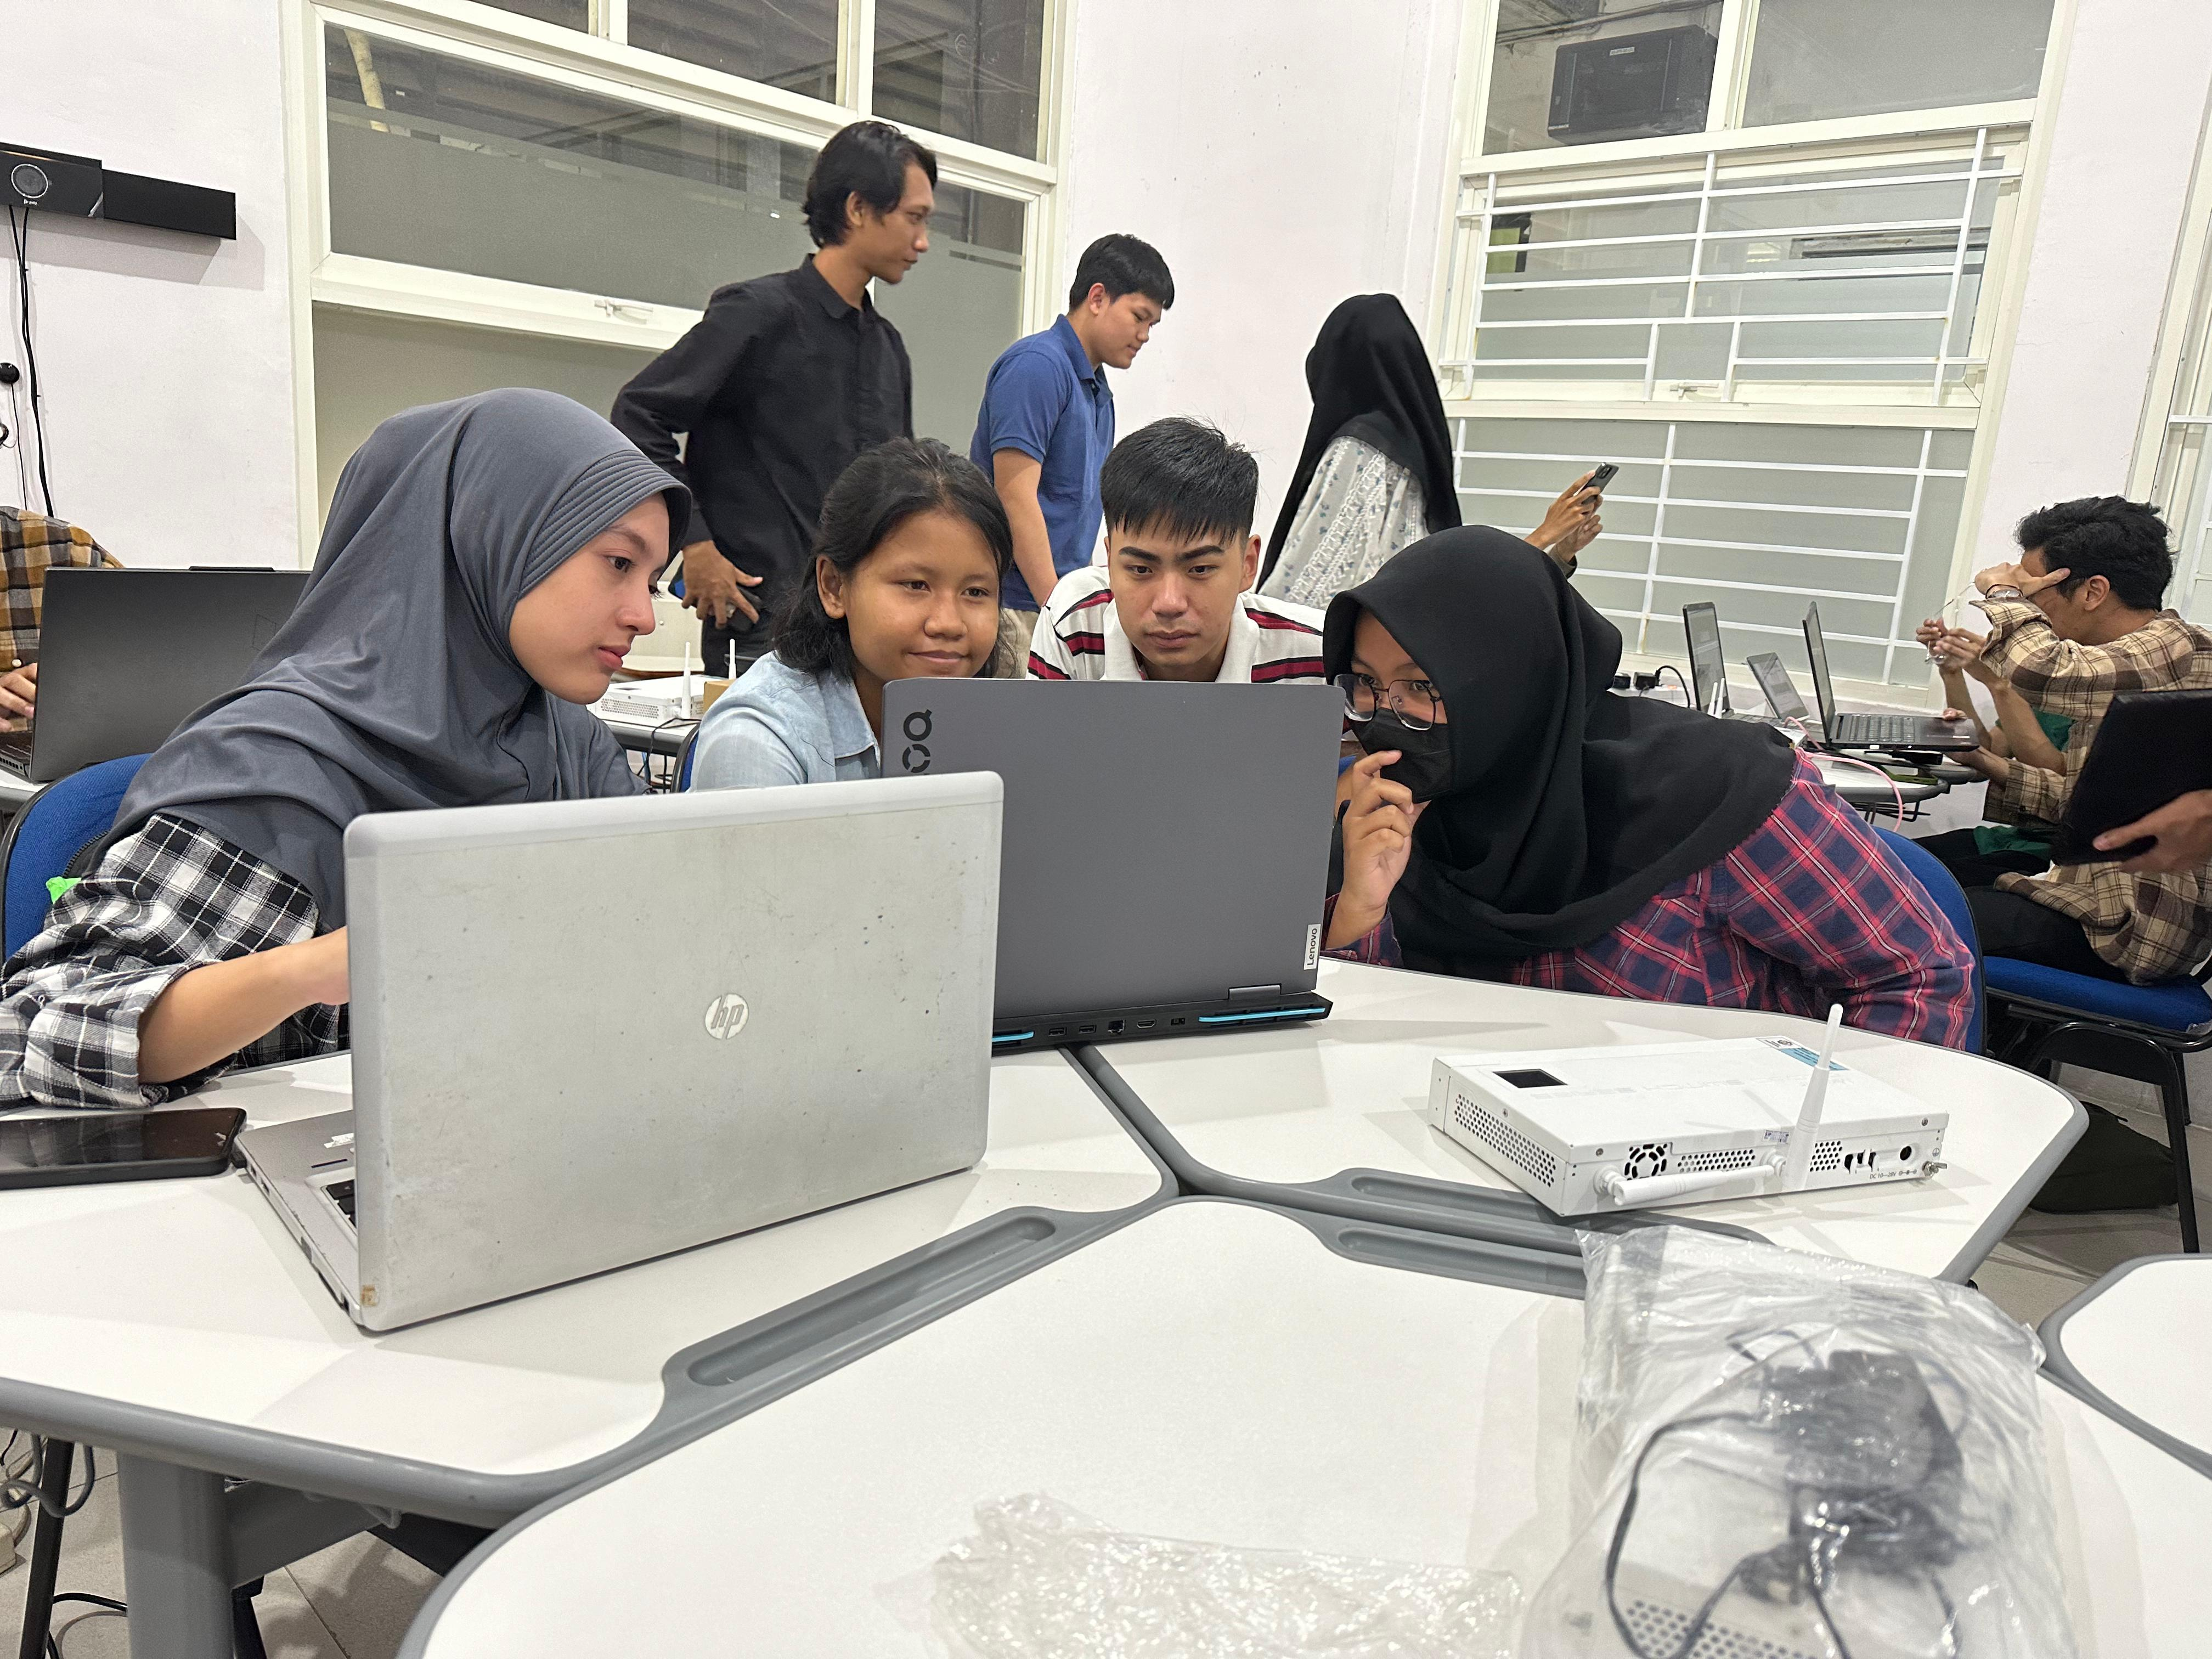
\includegraphics[width=0.75\linewidth]{P2/img/dokum1.jpg}
	\caption{Dokumentasi saat praktikum}
	\label{fig:gambar32}
\end{figure}